% Options for packages loaded elsewhere
\PassOptionsToPackage{unicode}{hyperref}
\PassOptionsToPackage{hyphens}{url}
\PassOptionsToPackage{dvipsnames,svgnames,x11names}{xcolor}
%
\documentclass[a4paper,12pt]{article}
\usepackage[notransparent]{svg}
\usepackage[utf8]{inputenc}
\usepackage[lmargin=3cm,tmargin=3cm,rmargin=2cm,bmargin=2cm]{geometry}
\usepackage{fancyhdr}
\usepackage{orcidlink}
\fancyhf{}
\fancyhead[R]{\thepage}
\renewcommand{\headrulewidth}{0pt}
\usepackage[onehalfspacing]{setspace}
\usepackage{blindtext}
\usepackage[T1]{fontenc}
% \usepackage[brazil]{babel}
\usepackage[document]{ragged2e}
\usepackage{pdflscape}
\usepackage{pdfpages}
\usepackage{float}
\usepackage{changepage}

\usepackage{graphicx, xcolor, comment, enumerate, multirow, multicol}
\usepackage{indentfirst}

\usepackage{amsfonts, amsthm, amsmath, amssymb, dsfont, mathtools}
\usepackage{tikz, tkz-base, tkz-fct}
\usepackage[style=abnt]{biblatex}

\usepackage{titlesec}
\usepackage{adjustbox}
\usepackage[skip=5pt, indent=15pt]{parskip}

\titleformat{\section}
{\normalsize\bfseries}{\thesection.}{1em}{}
\titleformat{\subsection}
{\normalsize}{\thesubsection.}{1em}{}
\titleformat{\subsubsection}
{\normalsize}{\thesubsubsection.}{1em}{}

\newcommand{\PR}[1]{\ensuremath{\left[#1\right]}}
\newcommand{\PC}[1]{\ensuremath{\left(#1\right)}}
\newcommand{\chav}[1]{\ensuremath{\left\{#1\right\}}}
\newcommand{\system}[1]{\ensuremath{\left\{#1\right}}
\newcommand{\floor}[1]{\ensuremath{\left \lfloor #1\right \rfloor}}
\newcommand{\FontTable}[1]{\vspace{-\baselineskip}\begin{footnotesize}#1\end{footnotesize}}

% Citacao direta com mais de 3 linhas - ABNT NBR 10520/2002 - 5.3
\newlength{\ABNTEXcitacaorecuo}% recuo de 4 cm da margem esquerda
\setlength{\ABNTEXcitacaorecuo}{4cm}
\newcommand{\ABNTEXfontereduzida}{\footnotesize}
\newenvironment*{citacao}[1][default]{%
   \list{}%
   \ABNTEXfontereduzida%
   \addtolength{\leftskip}{\ABNTEXcitacaorecuo}%
   \item[]%
   \singlespacing
   \ifthenelse{\not\equal{#1}{default}}{\itshape\selectlanguage{#1}}{}%
 }{%
   \endlist}%
% ---


% Citacao direta com mais de 3 linhas - ABNT NBR 10520/2002 - 5.3
\newlength{\aprovacao}% recuo de 4 cm da margem esquerda
\setlength{\aprovacao}{10.5cm}
\newcommand{\aprovacaofonte}{\normalsize}
\newenvironment*{citacao2}[1][default]{%
   \list{}%
   \aprovacaofonte%
   \addtolength{\leftskip}{\aprovacao}%
   \item[]%
   \singlespacing
   \justify
   \ifthenelse{\not\equal{#1}{default}}{\itshape\selectlanguage{#1}}{}%
 }{%
   \endlist}%
% ---


\newcommand{\fig}[4]{%
  \begin{figure}[H]
    \centering
    \caption{#1}
    \label{#2}
    \includegraphics{#3}
    
    \vspace{0.5cm}
    
    \begin{footnotesize}
      Fonte: #4
    \end{footnotesize}
  \end{figure}
}

\newcommand{\quadro}[4]{%
  \renewcommand{\figurename}{Quadro}
  \setcounter{figure}{0}
  \begin{figure}[H]
    \captionsetup{list=no}
    \centering
    \caption{#1}
    \label{#2}
    \includegraphics{#3}
    
    \vspace{0.5cm}
    
    \begin{footnotesize}
      Fonte: #4
    \end{footnotesize}
  \end{figure}
}

\newenvironment{invisible}{\color{white}}{}

\usepackage{amsmath,amssymb}
\usepackage{iftex}
\ifPDFTeX
  \usepackage[T1]{fontenc}
  \usepackage[utf8]{inputenc}
  \usepackage{textcomp} % provide euro and other symbols
\else % if luatex or xetex
  \usepackage{unicode-math}
  \defaultfontfeatures{Scale=MatchLowercase}
  \defaultfontfeatures[\rmfamily]{Ligatures=TeX,Scale=1}
\fi
\usepackage{lmodern}
\ifPDFTeX\else  
    % xetex/luatex font selection
  \setmainfont[]{Times New Roman}
\fi
% Use upquote if available, for straight quotes in verbatim environments
\IfFileExists{upquote.sty}{\usepackage{upquote}}{}
\IfFileExists{microtype.sty}{% use microtype if available
  \usepackage[]{microtype}
  \UseMicrotypeSet[protrusion]{basicmath} % disable protrusion for tt fonts
}{}
\makeatletter
\@ifundefined{KOMAClassName}{% if non-KOMA class
  \IfFileExists{parskip.sty}{%
    \usepackage{parskip}
  }{% else
    \setlength{\parindent}{0pt}
    \setlength{\parskip}{6pt plus 2pt minus 1pt}}
}{% if KOMA class
  \KOMAoptions{parskip=half}}
\makeatother
\usepackage{xcolor}
\setlength{\emergencystretch}{3em} % prevent overfull lines
\setcounter{secnumdepth}{-\maxdimen} % remove section numbering
% Make \paragraph and \subparagraph free-standing
\ifx\paragraph\undefined\else
  \let\oldparagraph\paragraph
  \renewcommand{\paragraph}[1]{\oldparagraph{#1}\mbox{}}
\fi
\ifx\subparagraph\undefined\else
  \let\oldsubparagraph\subparagraph
  \renewcommand{\subparagraph}[1]{\oldsubparagraph{#1}\mbox{}}
\fi

\usepackage{color}
\usepackage{fancyvrb}
\newcommand{\VerbBar}{|}
\newcommand{\VERB}{\Verb[commandchars=\\\{\}]}
\DefineVerbatimEnvironment{Highlighting}{Verbatim}{commandchars=\\\{\}}
% Add ',fontsize=\small' for more characters per line
\usepackage{framed}
\definecolor{shadecolor}{RGB}{255,255,255}
\newenvironment{Shaded}{\begin{snugshade}}{\end{snugshade}}
\newcommand{\AlertTok}[1]{\textcolor[rgb]{0.75,0.01,0.01}{\textbf{\colorbox[rgb]{0.97,0.90,0.90}{#1}}}}
\newcommand{\AnnotationTok}[1]{\textcolor[rgb]{0.79,0.38,0.79}{#1}}
\newcommand{\AttributeTok}[1]{\textcolor[rgb]{0.00,0.34,0.68}{#1}}
\newcommand{\BaseNTok}[1]{\textcolor[rgb]{0.69,0.50,0.00}{#1}}
\newcommand{\BuiltInTok}[1]{\textcolor[rgb]{0.39,0.29,0.61}{\textbf{#1}}}
\newcommand{\CharTok}[1]{\textcolor[rgb]{0.57,0.30,0.62}{#1}}
\newcommand{\CommentTok}[1]{\textcolor[rgb]{0.54,0.53,0.53}{#1}}
\newcommand{\CommentVarTok}[1]{\textcolor[rgb]{0.00,0.58,1.00}{#1}}
\newcommand{\ConstantTok}[1]{\textcolor[rgb]{0.67,0.33,0.00}{#1}}
\newcommand{\ControlFlowTok}[1]{\textcolor[rgb]{0.12,0.11,0.11}{\textbf{#1}}}
\newcommand{\DataTypeTok}[1]{\textcolor[rgb]{0.00,0.34,0.68}{#1}}
\newcommand{\DecValTok}[1]{\textcolor[rgb]{0.69,0.50,0.00}{#1}}
\newcommand{\DocumentationTok}[1]{\textcolor[rgb]{0.38,0.47,0.50}{#1}}
\newcommand{\ErrorTok}[1]{\textcolor[rgb]{0.75,0.01,0.01}{\underline{#1}}}
\newcommand{\ExtensionTok}[1]{\textcolor[rgb]{0.00,0.58,1.00}{\textbf{#1}}}
\newcommand{\FloatTok}[1]{\textcolor[rgb]{0.69,0.50,0.00}{#1}}
\newcommand{\FunctionTok}[1]{\textcolor[rgb]{0.39,0.29,0.61}{#1}}
\newcommand{\ImportTok}[1]{\textcolor[rgb]{1.00,0.33,0.00}{#1}}
\newcommand{\InformationTok}[1]{\textcolor[rgb]{0.69,0.50,0.00}{#1}}
\newcommand{\KeywordTok}[1]{\textcolor[rgb]{0.12,0.11,0.11}{\textbf{#1}}}
\newcommand{\NormalTok}[1]{\textcolor[rgb]{0.12,0.11,0.11}{#1}}
\newcommand{\OperatorTok}[1]{\textcolor[rgb]{0.12,0.11,0.11}{#1}}
\newcommand{\OtherTok}[1]{\textcolor[rgb]{0.00,0.43,0.16}{#1}}
\newcommand{\PreprocessorTok}[1]{\textcolor[rgb]{0.00,0.43,0.16}{#1}}
\newcommand{\RegionMarkerTok}[1]{\textcolor[rgb]{0.00,0.34,0.68}{\colorbox[rgb]{0.88,0.91,0.97}{#1}}}
\newcommand{\SpecialCharTok}[1]{\textcolor[rgb]{0.24,0.68,0.91}{#1}}
\newcommand{\SpecialStringTok}[1]{\textcolor[rgb]{1.00,0.33,0.00}{#1}}
\newcommand{\StringTok}[1]{\textcolor[rgb]{0.75,0.01,0.01}{#1}}
\newcommand{\VariableTok}[1]{\textcolor[rgb]{0.00,0.34,0.68}{#1}}
\newcommand{\VerbatimStringTok}[1]{\textcolor[rgb]{0.75,0.01,0.01}{#1}}
\newcommand{\WarningTok}[1]{\textcolor[rgb]{0.75,0.01,0.01}{#1}}

\providecommand{\tightlist}{%
  \setlength{\itemsep}{0pt}\setlength{\parskip}{0pt}}\usepackage{longtable,booktabs,array}
\usepackage{calc} % for calculating minipage widths
% Correct order of tables after \paragraph or \subparagraph
\usepackage{etoolbox}
\makeatletter
\patchcmd\longtable{\par}{\if@noskipsec\mbox{}\fi\par}{}{}
\makeatother
% Allow footnotes in longtable head/foot
\IfFileExists{footnotehyper.sty}{\usepackage{footnotehyper}}{\usepackage{footnote}}
\makesavenoteenv{longtable}
\usepackage{graphicx}
\makeatletter
\def\maxwidth{\ifdim\Gin@nat@width>\linewidth\linewidth\else\Gin@nat@width\fi}
\def\maxheight{\ifdim\Gin@nat@height>\textheight\textheight\else\Gin@nat@height\fi}
\makeatother
% Scale images if necessary, so that they will not overflow the page
% margins by default, and it is still possible to overwrite the defaults
% using explicit options in \includegraphics[width, height, ...]{}
\setkeys{Gin}{width=\maxwidth,height=\maxheight,keepaspectratio}
% Set default figure placement to htbp
\makeatletter
\def\fps@figure{htbp}
\makeatother
\newlength{\cslhangindent}
\setlength{\cslhangindent}{1.5em}
\newlength{\csllabelwidth}
\setlength{\csllabelwidth}{3em}
\newlength{\cslentryspacingunit} % times entry-spacing
\setlength{\cslentryspacingunit}{\parskip}
\newenvironment{CSLReferences}[2] % #1 hanging-ident, #2 entry spacing
 {% don't indent paragraphs
  \setlength{\parindent}{0pt}
  % turn on hanging indent if param 1 is 1
  \ifodd #1
  \let\oldpar\par
  \def\par{\hangindent=\cslhangindent\oldpar}
  \fi
  % set entry spacing
  \setlength{\parskip}{#2\cslentryspacingunit}
 }%
 {}
\usepackage{calc}
\newcommand{\CSLBlock}[1]{#1\hfill\break}
\newcommand{\CSLLeftMargin}[1]{\parbox[t]{\csllabelwidth}{#1}}
\newcommand{\CSLRightInline}[1]{\parbox[t]{\linewidth - \csllabelwidth}{#1}\break}
\newcommand{\CSLIndent}[1]{\hspace{\cslhangindent}#1}

\DefineVerbatimEnvironment{Highlighting}{Verbatim}{commandchars=\\\{\},fontsize=\footnotesize}
\makeatletter
\makeatother
\makeatletter
\makeatother
\makeatletter
\@ifpackageloaded{caption}{}{\usepackage{caption}}
\AtBeginDocument{%
\ifdefined\contentsname
  \renewcommand*\contentsname{Índice}
\else
  \newcommand\contentsname{Índice}
\fi
\ifdefined\listfigurename
  \renewcommand*\listfigurename{Lista de Figuras}
\else
  \newcommand\listfigurename{Lista de Figuras}
\fi
\ifdefined\listtablename
  \renewcommand*\listtablename{Lista de Tabelas}
\else
  \newcommand\listtablename{Lista de Tabelas}
\fi
\ifdefined\figurename
  \renewcommand*\figurename{Figura}
\else
  \newcommand\figurename{Figura}
\fi
\ifdefined\tablename
  \renewcommand*\tablename{Tabela}
\else
  \newcommand\tablename{Tabela}
\fi
}
\@ifpackageloaded{float}{}{\usepackage{float}}
\floatstyle{ruled}
\@ifundefined{c@chapter}{\newfloat{codelisting}{h}{lop}}{\newfloat{codelisting}{h}{lop}[chapter]}
\floatname{codelisting}{Listagem}
\newcommand*\listoflistings{\listof{codelisting}{Lista de Listagens}}
\makeatother
\makeatletter
\@ifpackageloaded{caption}{}{\usepackage{caption}}
\@ifpackageloaded{subcaption}{}{\usepackage{subcaption}}
\makeatother
\makeatletter
\makeatother
\ifLuaTeX
\usepackage[bidi=basic]{babel}
\else
\usepackage[bidi=default]{babel}
\fi
\babelprovide[main,import]{brazilian}
% get rid of language-specific shorthands (see #6817):
\let\LanguageShortHands\languageshorthands
\def\languageshorthands#1{}
\ifLuaTeX
  \usepackage{selnolig}  % disable illegal ligatures
\fi
\IfFileExists{bookmark.sty}{\usepackage{bookmark}}{\usepackage{hyperref}}
\IfFileExists{xurl.sty}{\usepackage{xurl}}{} % add URL line breaks if available
\urlstyle{same} % disable monospaced font for URLs
\hypersetup{
  pdftitle={MÍNIMOS QUADRADOS ORDINÁRIOS: UMA APLICAÇÃO NA ANÁLISE DAS QUESTÕES INSTITUCIONAIS DE MUNICÍPIOS BRASILEIROS},
  pdfauthor={Flávio Hugo Pangracio Silva; Guilherme Gomes Ferreira},
  pdflang={pt-BR},
  colorlinks=true,
  linkcolor={blue},
  filecolor={Maroon},
  citecolor={Blue},
  urlcolor={Blue},
  pdfcreator={LaTeX via pandoc}}

\title{MÍNIMOS QUADRADOS ORDINÁRIOS: UMA APLICAÇÃO NA ANÁLISE DAS
QUESTÕES INSTITUCIONAIS DE MUNICÍPIOS BRASILEIROS}
\author{Flávio Hugo Pangracio Silva \and Guilherme Gomes Ferreira}
\date{}

\begin{document}
% Capa
\thispagestyle{empty}
\pagenumbering{roman}

\begin{center}
UNIVERSIDADE FEDERAL DE MINAS GERAIS
\end{center}


\vspace{3.5cm}

\begin{center}
    \textbf{MÍNIMOS QUADRADOS ORDINÁRIOS: UMA APLICAÇÃO NA ANÁLISE DAS
QUESTÕES INSTITUCIONAIS DE MUNICÍPIOS BRASILEIROS}
\end{center}

\vspace{3.5cm}
\hypersetup{
    urlcolor=black,
    linkcolor=black
}

\begin{center}
Flávio Hugo Pangracio
Silva~\orcidlink{0000-0003-4045-101X}\\flaviopangracio@cedeplar.ufmg.br\\\href{https://cedeplar.ufmg.br}{Cedeplar
- UFMG}\\\vspace{1cm}Guilherme Gomes
Ferreira~\orcidlink{0009-0006-5032-8997}\\guilhermegf2019@cedeplar.ufmg.br\\\href{https://cedeplar.ufmg.br}{Cedeplar
- UFMG}\\\vspace{1cm}
\end{center}


\vspace{3.5cm}

\begin{center}

DOCENTE: Ana Hermeto.
\end{center}

\vspace{3.5cm}

\begin{center}

Belo Horizonte - MG

Abril - 2024
    
\end{center}

\newpage

% Lista de figuras
\renewcommand{\listfigurename}{LISTA DE FIGURAS}
\pagestyle{fancy}
\listoffigures

\newpage
% Lista de tabelas
\renewcommand{\listtablename}{LISTA DE TABELAS}
\pagestyle{fancy}
\listoftables

\newpage
% Sumário
\renewcommand{\contentsname}{SUMÁRIO}
\pagestyle{fancy}
\tableofcontents

\titleformat{\section}{\normalsize\bfseries}{\thesection.}{1em}{}
\newpage
\pagenumbering{arabic}\pagestyle{fancy} \justify \onehalfspacing

\hypertarget{introduuxe7uxe3o}{%
\section{INTRODUÇÃO}\label{introduuxe7uxe3o}}

O presente trabalho se propõe a explorar de maneira detalhada o método
de mínimos quadrados ordinários (MQO), apresentando uma aplicação na
análise das questões institucionais presentes nos municípios
brasileiros. Este método estatístico é amplamente utilizado na análise
econômica, sendo fundamental para compreender as relações entre
variáveis e realizar previsões.

A escolha desse enfoque se justifica pela relevância crescente do estudo
das instituições no contexto municipal brasileiro, visto que as
políticas públicas e a gestão eficiente dessas instituições desempenham
um papel fundamental no desenvolvimento socioeconômico local. Nesse
sentido, compreender como diferentes variáveis institucionais estão
relacionadas entre si e como influenciam indicadores de crescimento e
desenvolvimento municipal torna-se uma questão de interesse.

Por meio deste trabalho, pretendemos não apenas apresentar a aplicação
prática do modelo de MQO, mas também fornecer uma base sólida de
compreensão teórica, destacando os fundamentos matemáticos e
estatísticos subjacentes a esse método. Para isso, organizaremos o
conteúdo em várias seções, nas quais abordaremos desde os princípios
básicos da regressão linear até aspectos mais avançados, passando pela
discussão sobre a formulação teórica do modelo de MQO.

Inicialmente, abordaremos os principais conceitos e definições
relacionados à regressão linear, discutindo os pressupostos e as
limitações desse modelo estatístico. Posteriormente, dedicaremos atenção
especial à formulação teórica do modelo de MQO, descrevendo o processo
de estimativa dos parâmetros e apresentando as principais propriedades
estatísticas dos estimadores obtidos por esse método. Além disso,
discutiremos técnicas de diagnóstico e avaliação da qualidade do modelo,
destacando a importância da interpretação correta dos resultados
obtidos.

Por fim, demonstraremos a aplicação do modelo de MQO na análise das
questões institucionais de municípios brasileiros, utilizando dados da
REGIC para ilustrar o processo de formulação, estimação e interpretação
do modelo. Espera-se que este trabalho contribua para ampliar o
entendimento sobre o método de MQO e sua aplicação.

\hypertarget{estimauxe7uxe3o}{%
\section{Estimação}\label{estimauxe7uxe3o}}

Carregando pacotes:

\begin{Shaded}
\begin{Highlighting}[]
\FunctionTok{library}\NormalTok{(readxl)}
\FunctionTok{library}\NormalTok{(dplyr)}
\end{Highlighting}
\end{Shaded}

Carregando a base da REGIC 2018 e ajustando as variáveis de interesse:

\begin{Shaded}
\begin{Highlighting}[]
\NormalTok{df\_regic }\OtherTok{\textless{}{-}}\NormalTok{ readxl}\SpecialCharTok{::}\FunctionTok{read\_xlsx}\NormalTok{(}
  \AttributeTok{path =} \StringTok{"data/REGIC2018 Cidades v2.xlsx"}\NormalTok{,}
  \AttributeTok{sheet=}\StringTok{"Base de dados por Cidades"}
\NormalTok{) }\SpecialCharTok{|\textgreater{}}
\NormalTok{  dplyr}\SpecialCharTok{::}\FunctionTok{filter}\NormalTok{(}
\NormalTok{    UF }\SpecialCharTok{==} \StringTok{"MG"}
\NormalTok{  ) }\SpecialCharTok{|\textgreater{}}
\NormalTok{  dplyr}\SpecialCharTok{::}\FunctionTok{select}\NormalTok{(}
    \StringTok{"COD\_CIDADE"}\NormalTok{,}
    \StringTok{"NOME\_CIDADE"}\NormalTok{,}
    \StringTok{"VAR01"}\NormalTok{,}
    \StringTok{"VAR03"}\NormalTok{,}
    \StringTok{"VAR23"}\NormalTok{,}
    \StringTok{"VAR29"}\NormalTok{,}
    \StringTok{"VAR85"}\NormalTok{,}
    \StringTok{"VAR89"}
\NormalTok{  ) }\SpecialCharTok{|\textgreater{}}
\NormalTok{  dplyr}\SpecialCharTok{::}\FunctionTok{rename}\NormalTok{(}
    \StringTok{"populacao"} \OtherTok{=} \StringTok{"VAR01"}\NormalTok{,}
    \StringTok{"pib"} \OtherTok{=} \StringTok{"VAR03"}\NormalTok{,}
    \StringTok{"cige"} \OtherTok{=} \StringTok{"VAR23"}\NormalTok{,}
    \StringTok{"cgp"} \OtherTok{=} \StringTok{"VAR29"}
\NormalTok{  ) }\SpecialCharTok{|\textgreater{}}
\NormalTok{  dplyr}\SpecialCharTok{::}\FunctionTok{mutate}\NormalTok{(}
    \StringTok{"populacao"} \OtherTok{=} \FunctionTok{as.numeric}\NormalTok{(populacao),}
    \StringTok{"pib"} \OtherTok{=} \FunctionTok{as.numeric}\NormalTok{(pib),}
    \StringTok{"cige"} \OtherTok{=} \FunctionTok{as.numeric}\NormalTok{(cige),}
    \StringTok{"cgp"} \OtherTok{=} \FunctionTok{as.numeric}\NormalTok{(cgp),}
    \StringTok{"banco\_publico"} \OtherTok{=} \FunctionTok{ifelse}\NormalTok{(VAR85 }\SpecialCharTok{|}\NormalTok{ VAR89, }\DecValTok{1}\NormalTok{, }\DecValTok{0}\NormalTok{),}
    \StringTok{"log\_cige"} \OtherTok{=} \FunctionTok{ifelse}\NormalTok{(}\FunctionTok{as.numeric}\NormalTok{(cige) }\SpecialCharTok{\textless{}} \DecValTok{1}\NormalTok{, }\DecValTok{0}\NormalTok{, }\FunctionTok{log}\NormalTok{(}\FunctionTok{as.numeric}\NormalTok{(cige))),}
    \StringTok{"log\_cgp"} \OtherTok{=} \FunctionTok{ifelse}\NormalTok{(}\FunctionTok{as.numeric}\NormalTok{(cgp) }\SpecialCharTok{\textless{}} \DecValTok{1}\NormalTok{, }\DecValTok{0}\NormalTok{, }\FunctionTok{log}\NormalTok{(}\FunctionTok{as.numeric}\NormalTok{(cgp)))}
\NormalTok{  )}

\NormalTok{df\_regic[}\FunctionTok{is.na}\NormalTok{(df\_regic)] }\OtherTok{\textless{}{-}} \DecValTok{0}

\NormalTok{df\_regic}\SpecialCharTok{$}\NormalTok{pib\_pc }\OtherTok{\textless{}{-}}\NormalTok{ df\_regic}\SpecialCharTok{$}\NormalTok{pib }\SpecialCharTok{/}\NormalTok{ df\_regic}\SpecialCharTok{$}\NormalTok{populacao}
\end{Highlighting}
\end{Shaded}

\hypertarget{anuxe1lise-descritiva}{%
\subsection{Análise Descritiva}\label{anuxe1lise-descritiva}}

\begin{Shaded}
\begin{Highlighting}[]
\DocumentationTok{\#\# PIB per capita}
\FunctionTok{hist}\NormalTok{(df\_regic}\SpecialCharTok{$}\NormalTok{pib\_pc, }\AttributeTok{freq=}\ConstantTok{FALSE}\NormalTok{, }\AttributeTok{ylim=}\FunctionTok{c}\NormalTok{(}\DecValTok{0}\NormalTok{,.}\DecValTok{07}\NormalTok{))}
\FunctionTok{lines}\NormalTok{(}\FunctionTok{density}\NormalTok{(df\_regic}\SpecialCharTok{$}\NormalTok{pib\_pc), }\AttributeTok{lwd=}\DecValTok{2}\NormalTok{)}
\end{Highlighting}
\end{Shaded}

\begin{figure}[H]

\caption{Histograma do PIB per capita}

{\centering 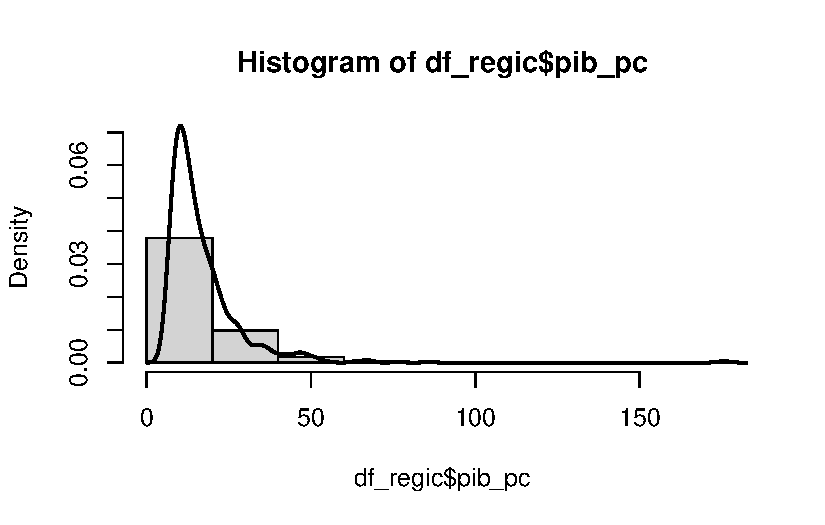
\includegraphics{main_files/figure-pdf/unnamed-chunk-3-1.pdf}

}

\end{figure}

\begin{Shaded}
\begin{Highlighting}[]
\FunctionTok{summary}\NormalTok{(df\_regic}\SpecialCharTok{$}\NormalTok{pib\_pc)}
\end{Highlighting}
\end{Shaded}

\begin{verbatim}
   Min. 1st Qu.  Median    Mean 3rd Qu.    Max. 
  5.388   9.945  13.484  17.128  19.856 177.101 
\end{verbatim}

\begin{Shaded}
\begin{Highlighting}[]
\FunctionTok{hist}\NormalTok{(df\_regic}\SpecialCharTok{$}\NormalTok{log\_cige, }\AttributeTok{freq=}\ConstantTok{FALSE}\NormalTok{)}
\FunctionTok{lines}\NormalTok{(}\FunctionTok{density}\NormalTok{(df\_regic}\SpecialCharTok{$}\NormalTok{log\_cige), }\AttributeTok{lwd=}\DecValTok{2}\NormalTok{)}
\end{Highlighting}
\end{Shaded}

\begin{figure}[H]

\caption{Coeficiente de Intensidade da Gestão Empresarial (CI)}

{\centering 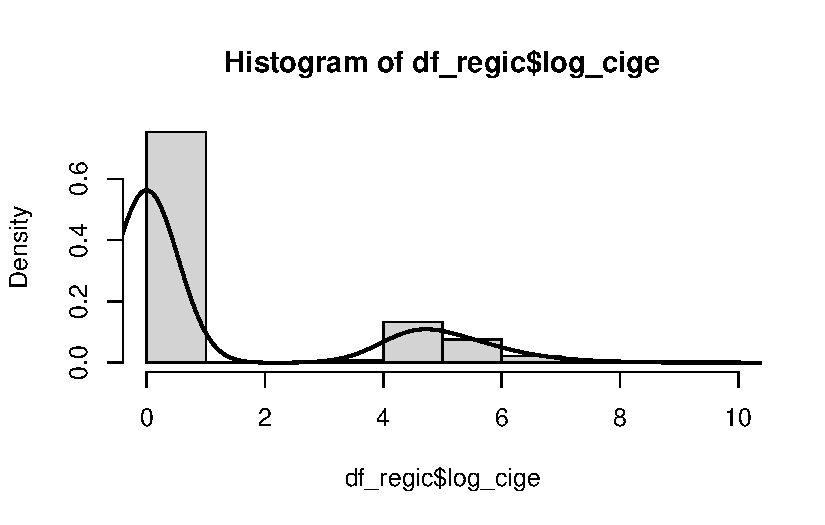
\includegraphics{main_files/figure-pdf/unnamed-chunk-5-1.pdf}

}

\end{figure}

\begin{Shaded}
\begin{Highlighting}[]
\FunctionTok{summary}\NormalTok{(df\_regic}\SpecialCharTok{$}\NormalTok{log\_cige)}
\end{Highlighting}
\end{Shaded}

\begin{verbatim}
   Min. 1st Qu.  Median    Mean 3rd Qu.    Max. 
  0.000   0.000   0.000   1.258   0.000   9.627 
\end{verbatim}

\begin{Shaded}
\begin{Highlighting}[]
\FunctionTok{hist}\NormalTok{(df\_regic}\SpecialCharTok{$}\NormalTok{log\_cgp, }\AttributeTok{freq=}\ConstantTok{FALSE}\NormalTok{)}
\FunctionTok{lines}\NormalTok{(}\FunctionTok{density}\NormalTok{(df\_regic}\SpecialCharTok{$}\NormalTok{log\_cgp), }\AttributeTok{lwd=}\DecValTok{2}\NormalTok{)}
\end{Highlighting}
\end{Shaded}

\begin{figure}[H]

\caption{Centralidade de Gestão Pública (CGP)}

{\centering 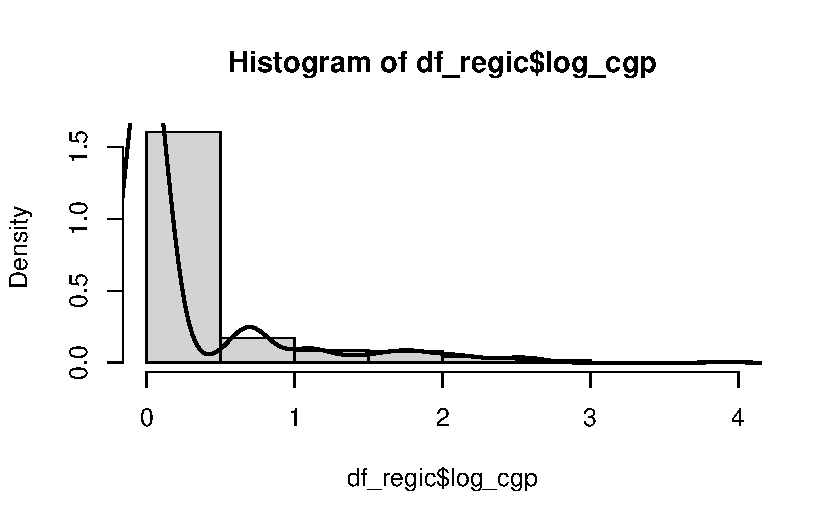
\includegraphics{main_files/figure-pdf/unnamed-chunk-7-1.pdf}

}

\end{figure}

\begin{Shaded}
\begin{Highlighting}[]
\FunctionTok{summary}\NormalTok{(df\_regic}\SpecialCharTok{$}\NormalTok{log\_cige)}
\end{Highlighting}
\end{Shaded}

\begin{verbatim}
   Min. 1st Qu.  Median    Mean 3rd Qu.    Max. 
  0.000   0.000   0.000   1.258   0.000   9.627 
\end{verbatim}

Heiss (2020) Greene (2019)

\newpage

\hypertarget{referuxeancias}{%
\section{REFERÊNCIAS}\label{referuxeancias}}

\singlespacing

\hypertarget{refs}{}
\begin{CSLReferences}{0}{1}
\leavevmode\vadjust pre{\hypertarget{ref-greene}{}}%
GREENE, W. H.
\textbf{\href{http://gen.lib.rus.ec/book/index.php?md5=2BB86D2F4CF47DB0A519E94D262C3331}{Econometric
Analysis Global Edition}}. 8. ed. {[}s.l.{]} Pearson-prentice Hall,
2019.

\leavevmode\vadjust pre{\hypertarget{ref-heiss}{}}%
HEISS, F.
\textbf{\href{http://gen.lib.rus.ec/book/index.php?md5=5C3417608D22D155EA90339688548999}{Using
R for Introductory Econometrics}}. 2. ed. {[}s.l: s.n.{]}.

\end{CSLReferences}



\end{document}
